\documentclass{article}\usepackage[]{graphicx}\usepackage[]{color}
%% maxwidth is the original width if it is less than linewidth
%% otherwise use linewidth (to make sure the graphics do not exceed the margin)
\makeatletter
\def\maxwidth{ %
  \ifdim\Gin@nat@width>\linewidth
    \linewidth
  \else
    \Gin@nat@width
  \fi
}
\makeatother

\definecolor{fgcolor}{rgb}{0.345, 0.345, 0.345}
\newcommand{\hlnum}[1]{\textcolor[rgb]{0.686,0.059,0.569}{#1}}%
\newcommand{\hlstr}[1]{\textcolor[rgb]{0.192,0.494,0.8}{#1}}%
\newcommand{\hlcom}[1]{\textcolor[rgb]{0.678,0.584,0.686}{\textit{#1}}}%
\newcommand{\hlopt}[1]{\textcolor[rgb]{0,0,0}{#1}}%
\newcommand{\hlstd}[1]{\textcolor[rgb]{0.345,0.345,0.345}{#1}}%
\newcommand{\hlkwa}[1]{\textcolor[rgb]{0.161,0.373,0.58}{\textbf{#1}}}%
\newcommand{\hlkwb}[1]{\textcolor[rgb]{0.69,0.353,0.396}{#1}}%
\newcommand{\hlkwc}[1]{\textcolor[rgb]{0.333,0.667,0.333}{#1}}%
\newcommand{\hlkwd}[1]{\textcolor[rgb]{0.737,0.353,0.396}{\textbf{#1}}}%
\let\hlipl\hlkwb

\usepackage{framed}
\makeatletter
\newenvironment{kframe}{%
 \def\at@end@of@kframe{}%
 \ifinner\ifhmode%
  \def\at@end@of@kframe{\end{minipage}}%
  \begin{minipage}{\columnwidth}%
 \fi\fi%
 \def\FrameCommand##1{\hskip\@totalleftmargin \hskip-\fboxsep
 \colorbox{shadecolor}{##1}\hskip-\fboxsep
     % There is no \\@totalrightmargin, so:
     \hskip-\linewidth \hskip-\@totalleftmargin \hskip\columnwidth}%
 \MakeFramed {\advance\hsize-\width
   \@totalleftmargin\z@ \linewidth\hsize
   \@setminipage}}%
 {\par\unskip\endMakeFramed%
 \at@end@of@kframe}
\makeatother

\definecolor{shadecolor}{rgb}{.97, .97, .97}
\definecolor{messagecolor}{rgb}{0, 0, 0}
\definecolor{warningcolor}{rgb}{1, 0, 1}
\definecolor{errorcolor}{rgb}{1, 0, 0}
\newenvironment{knitrout}{}{} % an empty environment to be redefined in TeX

\usepackage{alltt}
\usepackage{enumitem}
\usepackage{ amssymb }
\usepackage{ textcomp }
\usepackage{longtable}
\usepackage{amsmath,tabu}
\usepackage{caption}
\usepackage{subcaption}
\usepackage{float}
\usepackage[figurename=Supplemental Figure]{caption}
\usepackage{titling}

\setlength{\droptitle}{-5em}  
\topmargin=-0.4in
\evensidemargin=0in
\oddsidemargin=0in
\textwidth=6.5in
\textheight=9in
\headsep=0.25in

\title{Interrogation of human hematopoietic traits at single-cell and single-variant resolution}
\date{Supplemental Information}
\author{(Caleb, Erik, Jacob), Will?, Hilary, Joel, (Martin, Jason, Vijay)}
\IfFileExists{upquote.sty}{\usepackage{upquote}}{}
\begin{document}
\SweaveOpts{concordance=TRUE}
\maketitle
\section*{Overview of UK Biobank data}
\begin{enumerate}[label=(\Alph*)]
\item 



\begin{knitrout}
\definecolor{shadecolor}{rgb}{0.969, 0.969, 0.969}\color{fgcolor}\begin{figure}[H]

{\centering 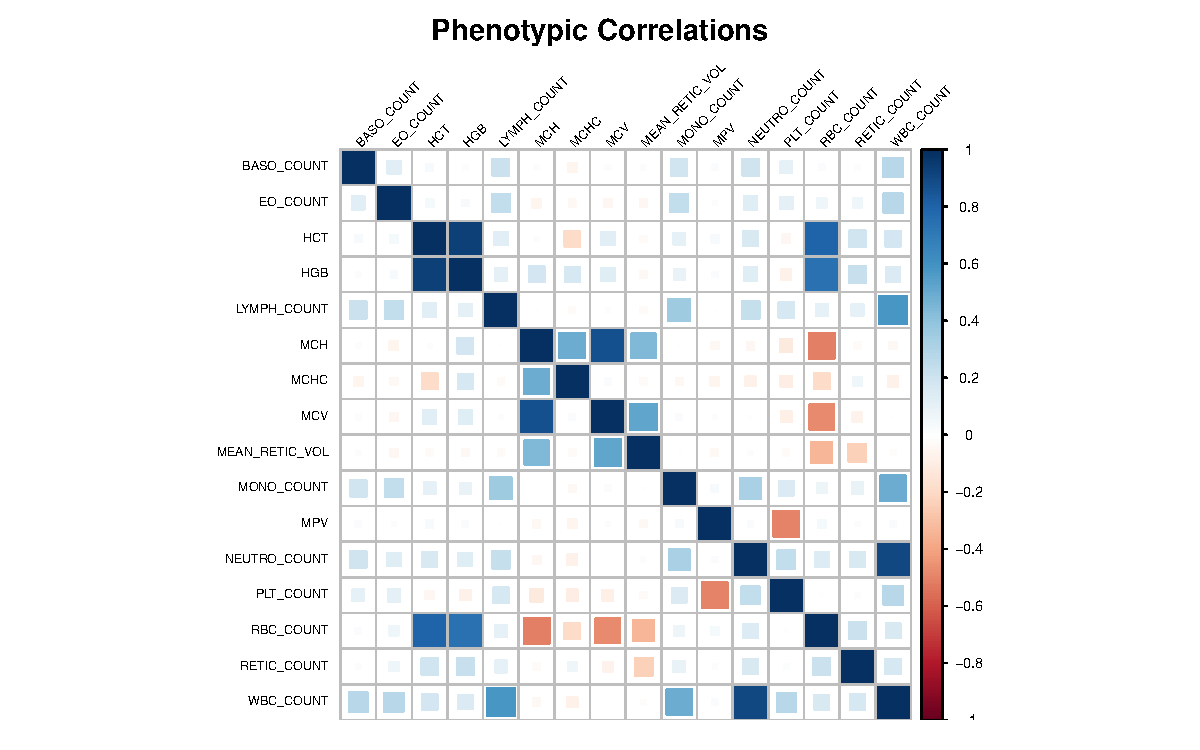
\includegraphics[width=\maxwidth]{figure/correlationPlots-1} 

}

\caption[Phenotypic and genetic correlations across the 16 traits examined]{Phenotypic and genetic correlations across the 16 traits examined. }\label{fig:correlationPlots}
\end{figure}


\end{knitrout}




\begin{knitrout}
\definecolor{shadecolor}{rgb}{0.969, 0.969, 0.969}\color{fgcolor}\begin{figure}[H]

{\centering 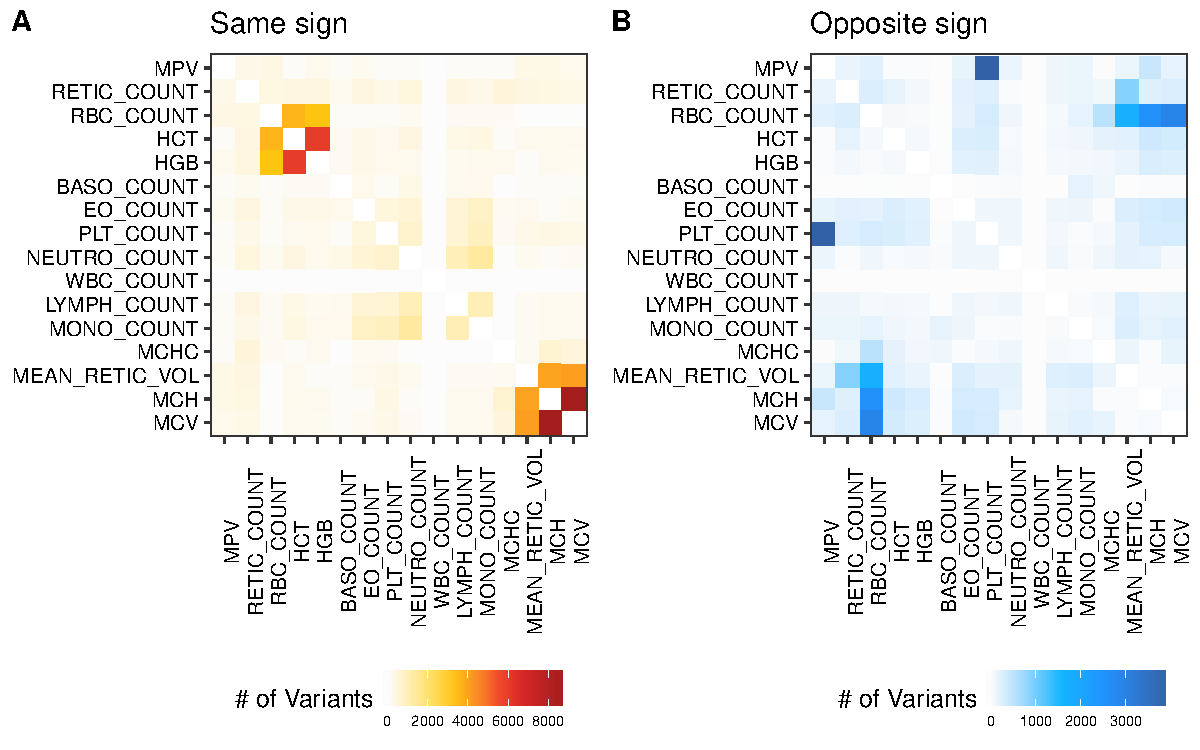
\includegraphics[width=\maxwidth]{figure/pleiotropyPlots-1} 

}

\caption[Numbers of pleiotropic variants]{Numbers of pleiotropic variants}\label{fig:pleiotropyPlots}
\end{figure}


\end{knitrout}

\begin{knitrout}
\definecolor{shadecolor}{rgb}{0.969, 0.969, 0.969}\color{fgcolor}\begin{figure}[H]

{\centering 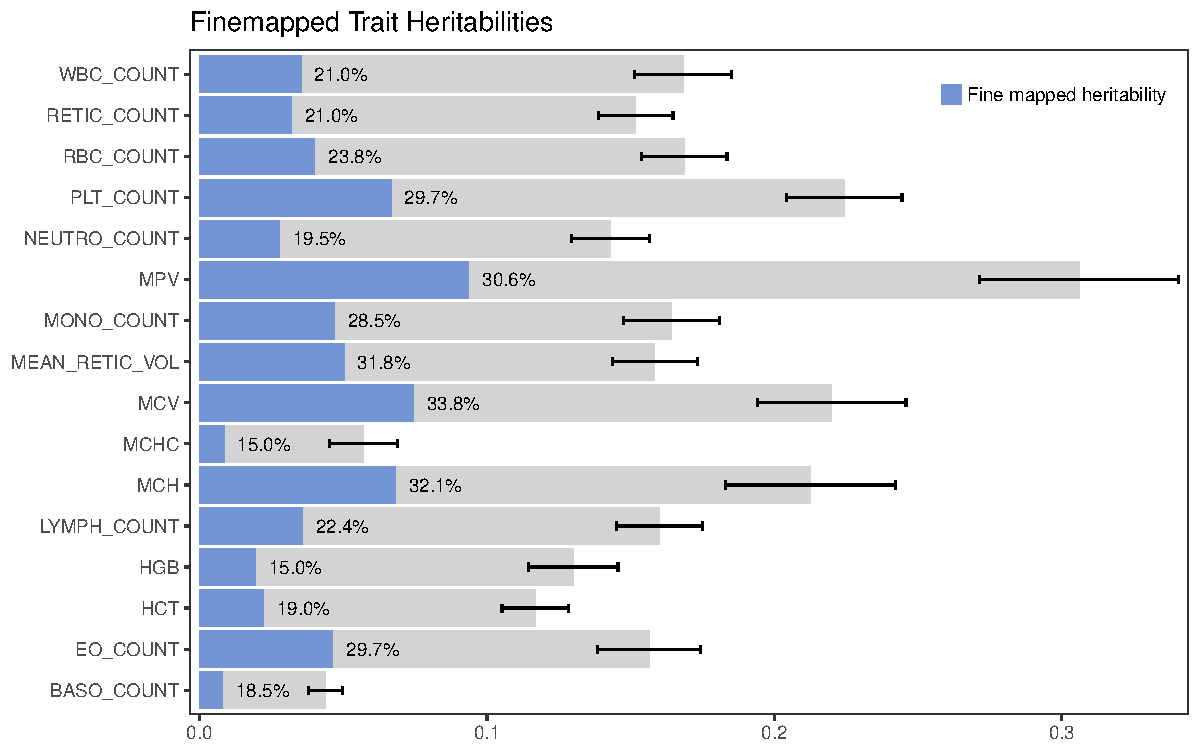
\includegraphics[width=\maxwidth]{figure/heritabilityPlots-1} 

}

\caption[Heritability estimates from LD Score Regression across 16 hematopoetic traits]{Heritability estimates from LD Score Regression across 16 hematopoetic traits. The estimates of the narrow-sense SNP heritabilities are plotted in gray with their corresponding standard erors. Heritability estimates for all variants with fine mapped posterior probability > 0.001 are plotted in blue for each trait, and the proportions of total narrow-sense heritability captured by these fine mapped variants (blue bar / gray bar) are indicated by the numbered labels.}\label{fig:heritabilityPlots}
\end{figure}


\end{knitrout}

\begin{knitrout}
\definecolor{shadecolor}{rgb}{0.969, 0.969, 0.969}\color{fgcolor}\begin{figure}[H]

{\centering 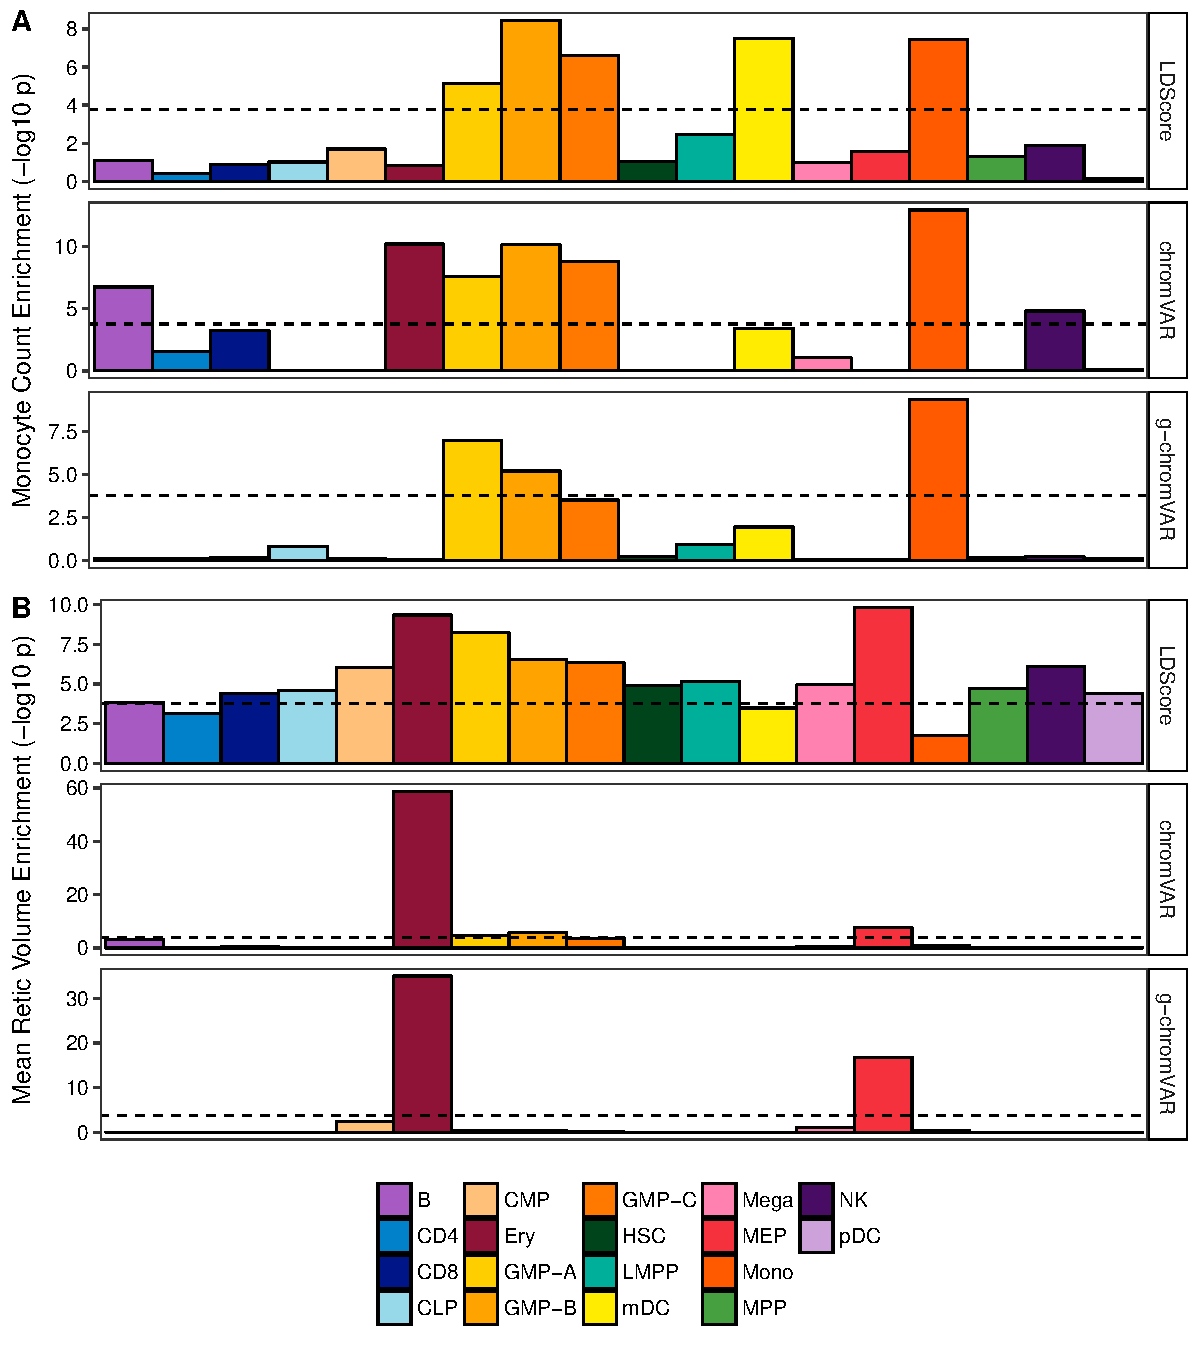
\includegraphics[width=\maxwidth]{figure/barplots-1} 

}

\caption[Hematopoetic cell type enrichments for Mean Retic Volume and Monocyte count using various methods]{Hematopoetic cell type enrichments for Mean Retic Volume and Monocyte count using various methods.}\label{fig:barplots}
\end{figure}


\end{knitrout}

\begin{knitrout}
\definecolor{shadecolor}{rgb}{0.969, 0.969, 0.969}\color{fgcolor}\begin{figure}[H]

{\centering 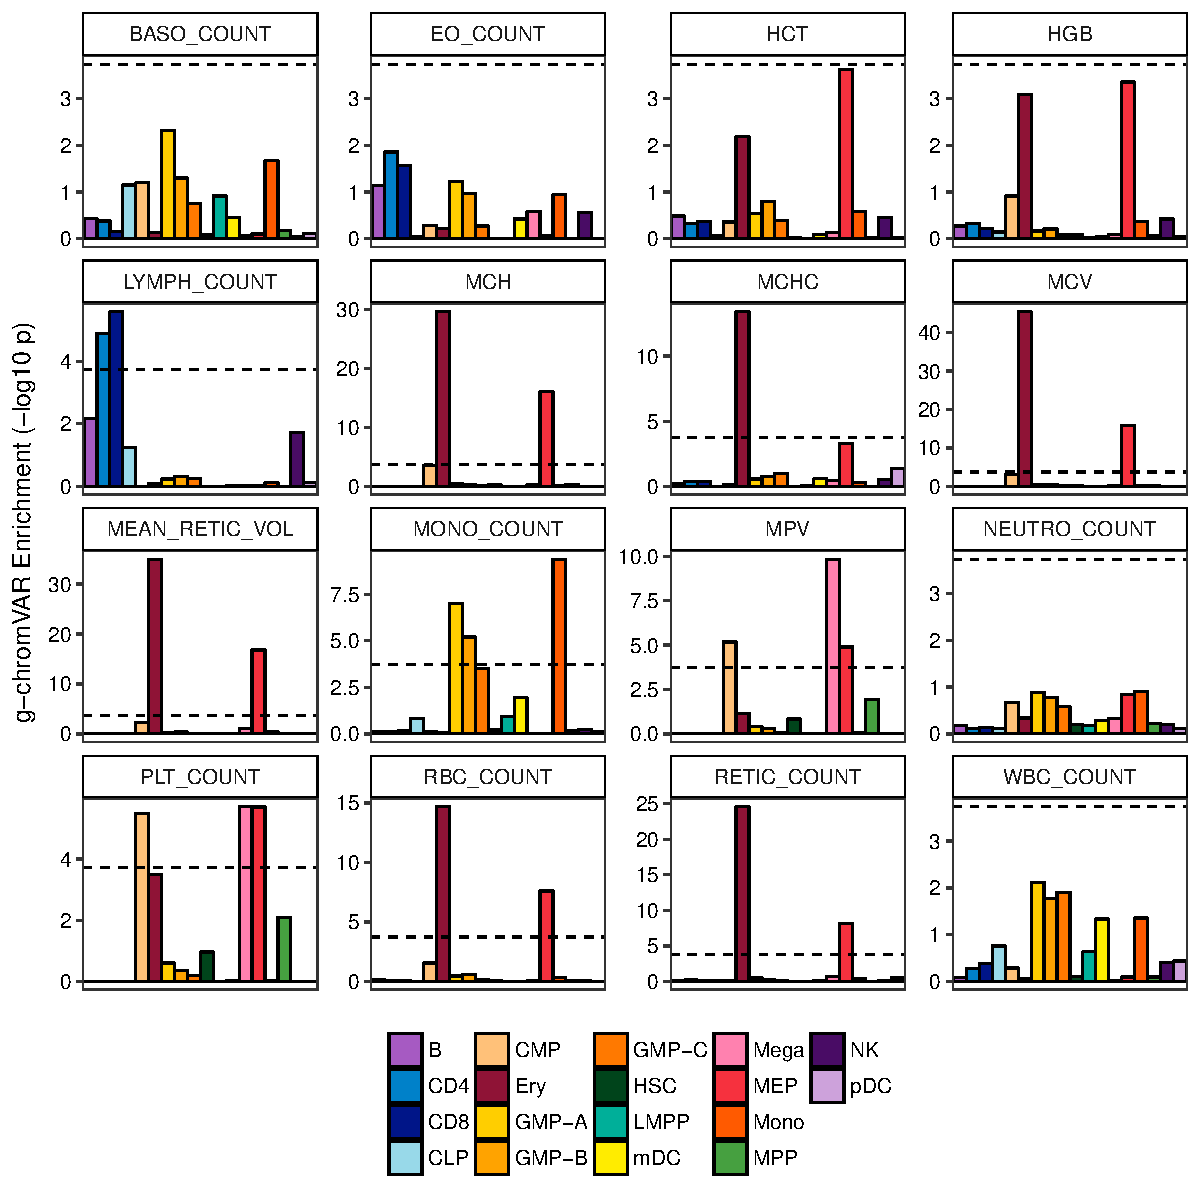
\includegraphics[width=\maxwidth]{figure/allGchromvar-1} 

}

\caption[All enrichments from g-chromVAR]{All enrichments from g-chromVAR. The horizontal line shows a Bonferonni multiple testing adjusted threshold for statistical significance of enrichment.}\label{fig:allGchromvar}
\end{figure}


\end{knitrout}

\begin{knitrout}
\definecolor{shadecolor}{rgb}{0.969, 0.969, 0.969}\color{fgcolor}\begin{figure}[H]

{\centering 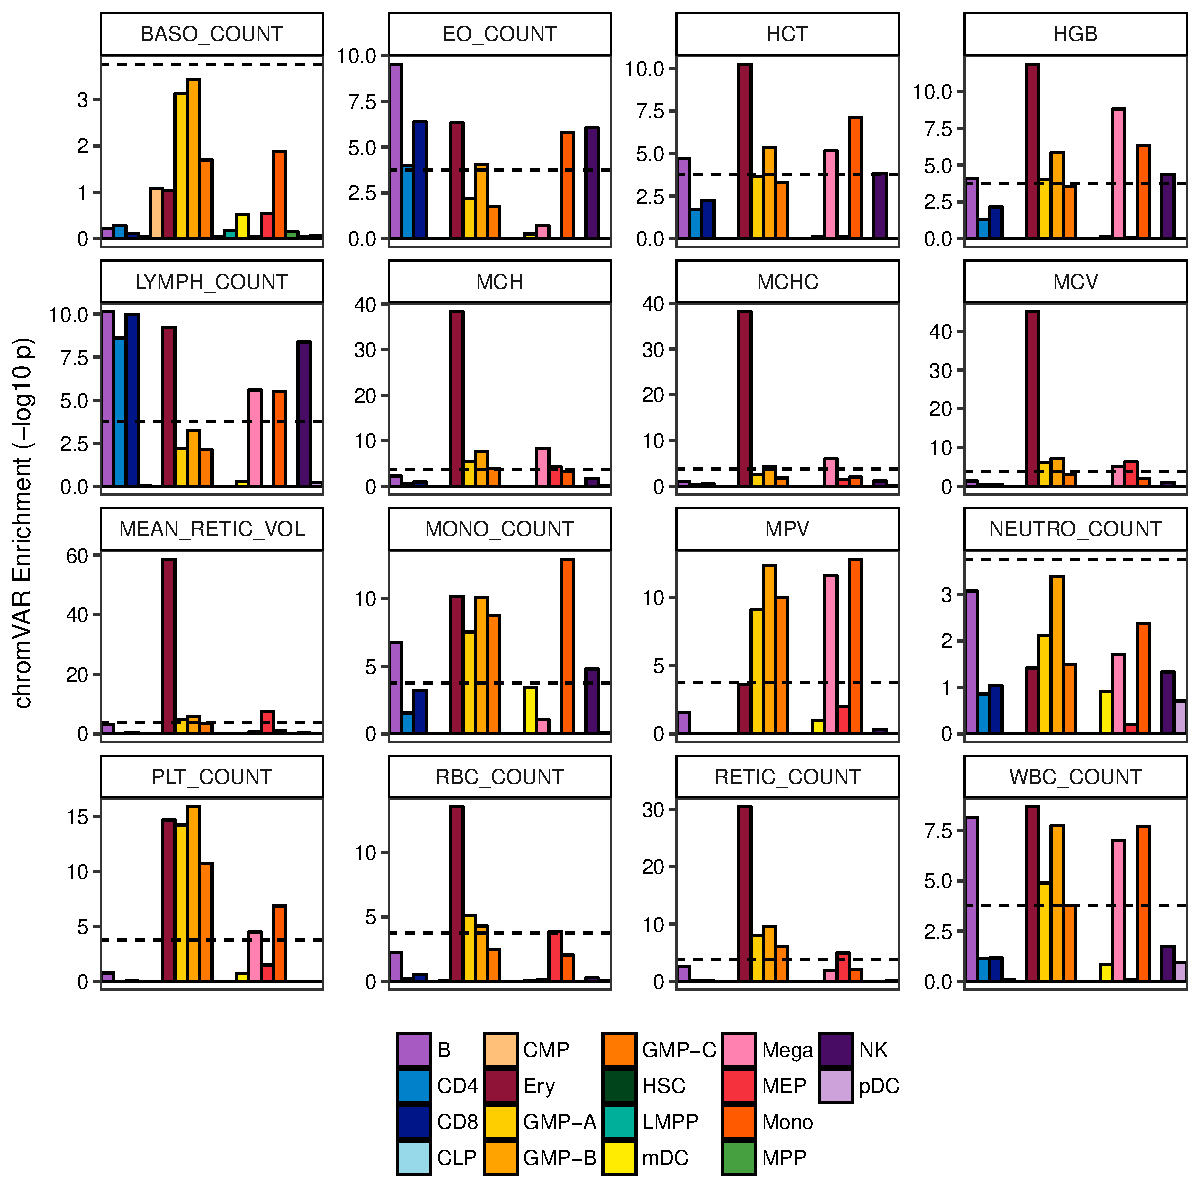
\includegraphics[width=\maxwidth]{figure/allchromVAR-1} 

}

\caption[All enrichments from chromVAR]{All enrichments from chromVAR. The horizontal line shows a Bonferonni multiple testing adjusted threshold for statistical significance of enrichment.}\label{fig:allchromVAR}
\end{figure}


\end{knitrout}

\begin{knitrout}
\definecolor{shadecolor}{rgb}{0.969, 0.969, 0.969}\color{fgcolor}\begin{figure}[H]

{\centering 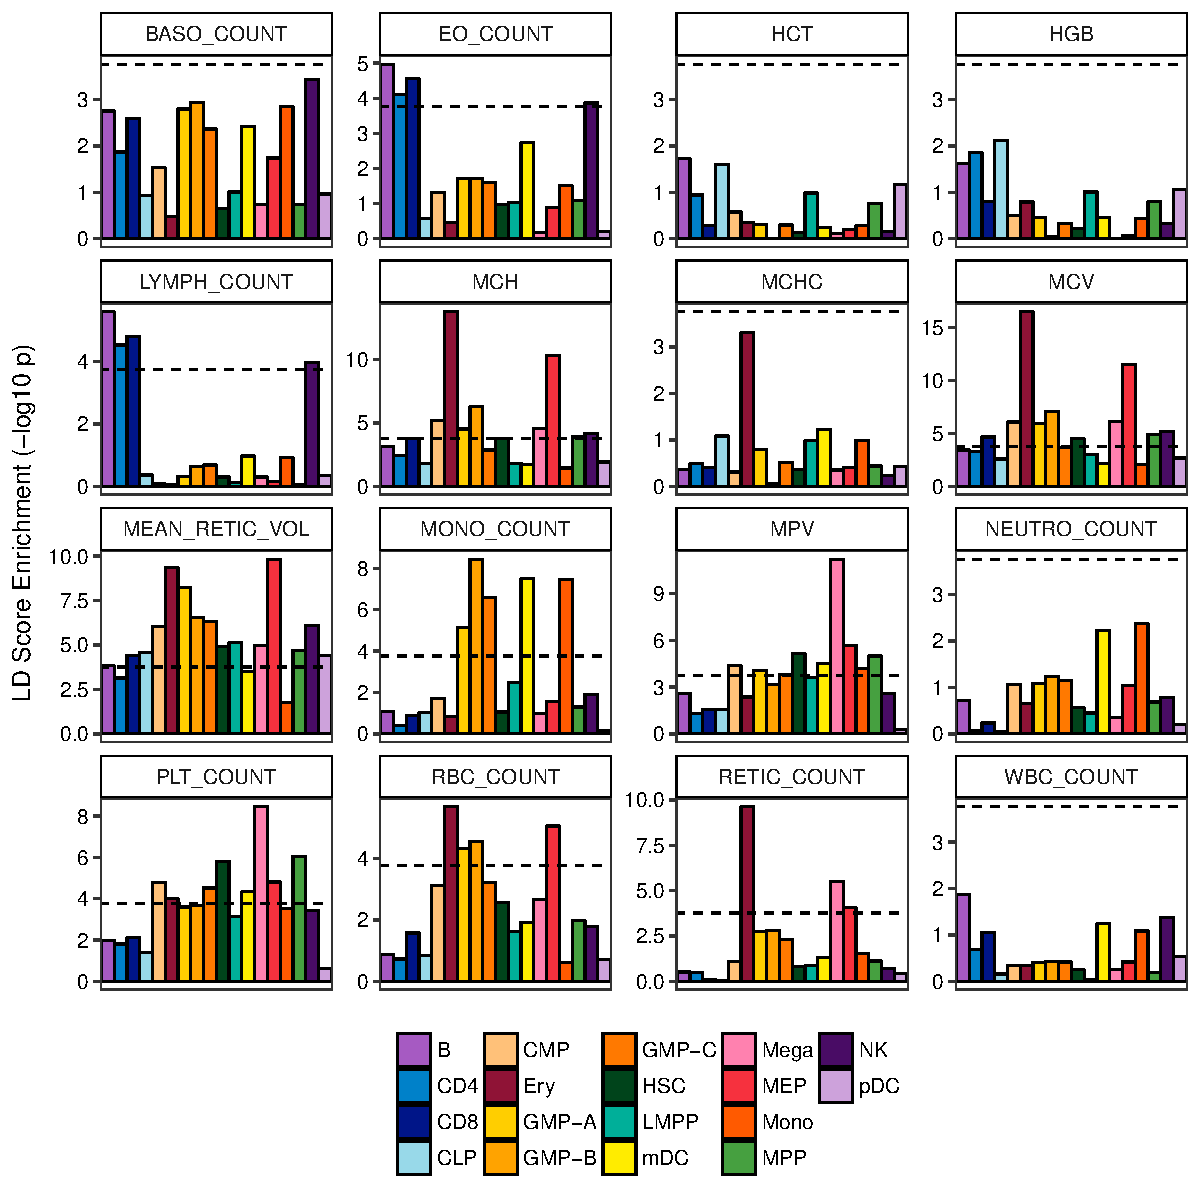
\includegraphics[width=\maxwidth]{figure/allLDscore-1} 

}

\caption[All enrichments from LD Score]{All enrichments from LD Score. The horizontal line shows a Bonferonni multiple testing adjusted threshold for statistical significance of enrichment.}\label{fig:allLDscore}
\end{figure}


\end{knitrout}

\begin{knitrout}
\definecolor{shadecolor}{rgb}{0.969, 0.969, 0.969}\color{fgcolor}\begin{figure}[H]

{\centering 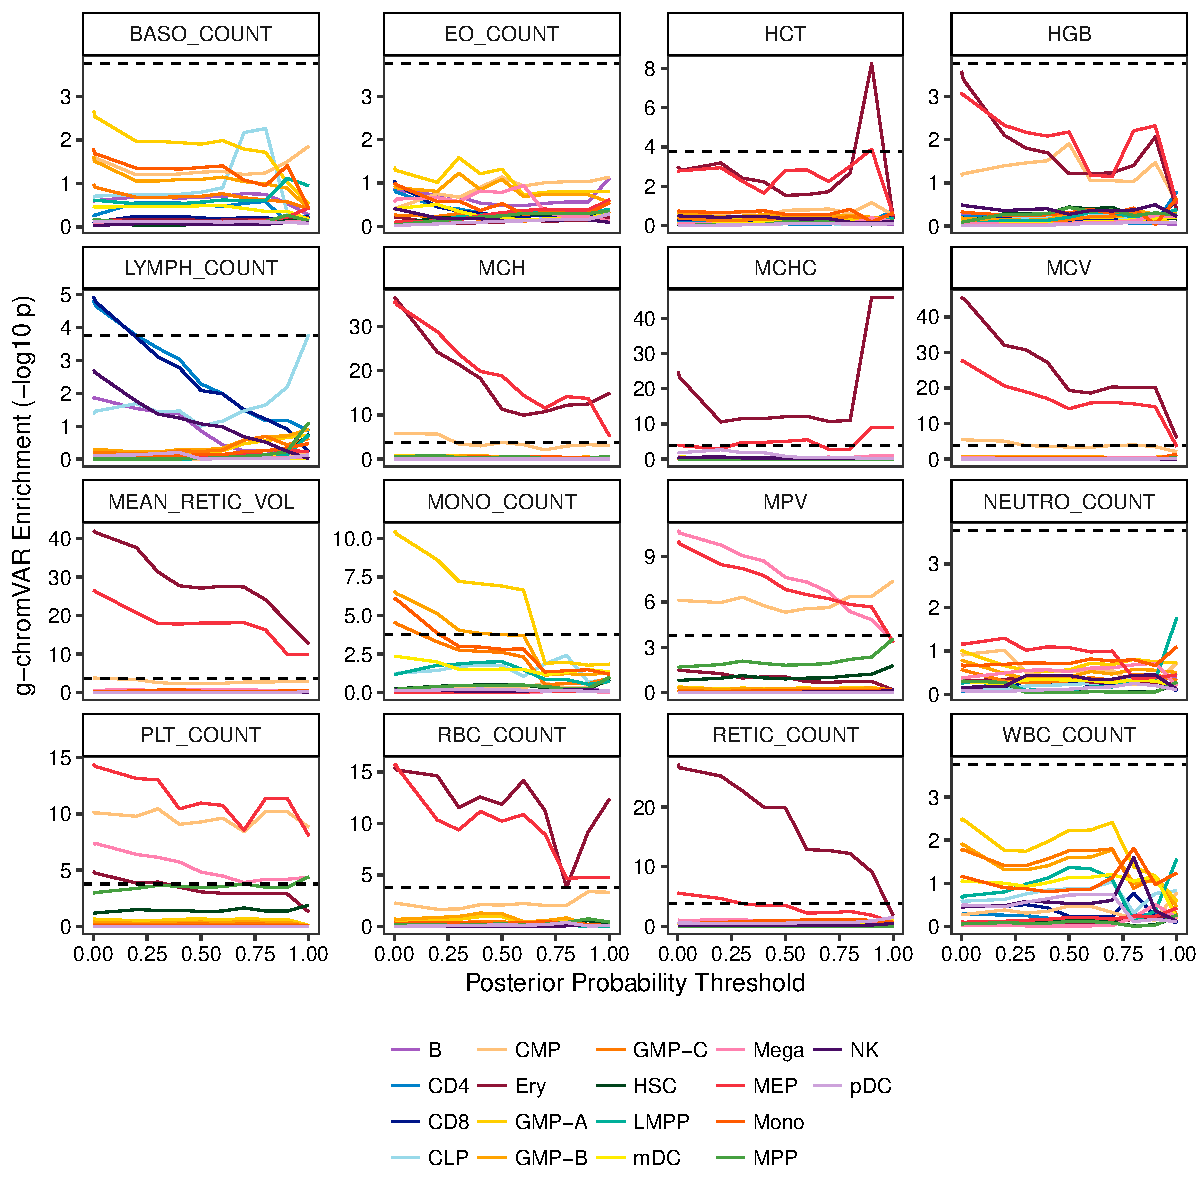
\includegraphics[width=\maxwidth]{figure/varyingPP-1} 

}

\caption[Cell type - trait enrichments for g-chromVAR across different finemap variants posterior probability cutoffs]{Cell type - trait enrichments for g-chromVAR across different finemap variants posterior probability cutoffs. The horizontal line shows a Bonferonni multiple testing adjusted threshold for statistical significance of enrichment.}\label{fig:varyingPP}
\end{figure}


\end{knitrout}
\item

\begin{figure}[H]
\centering
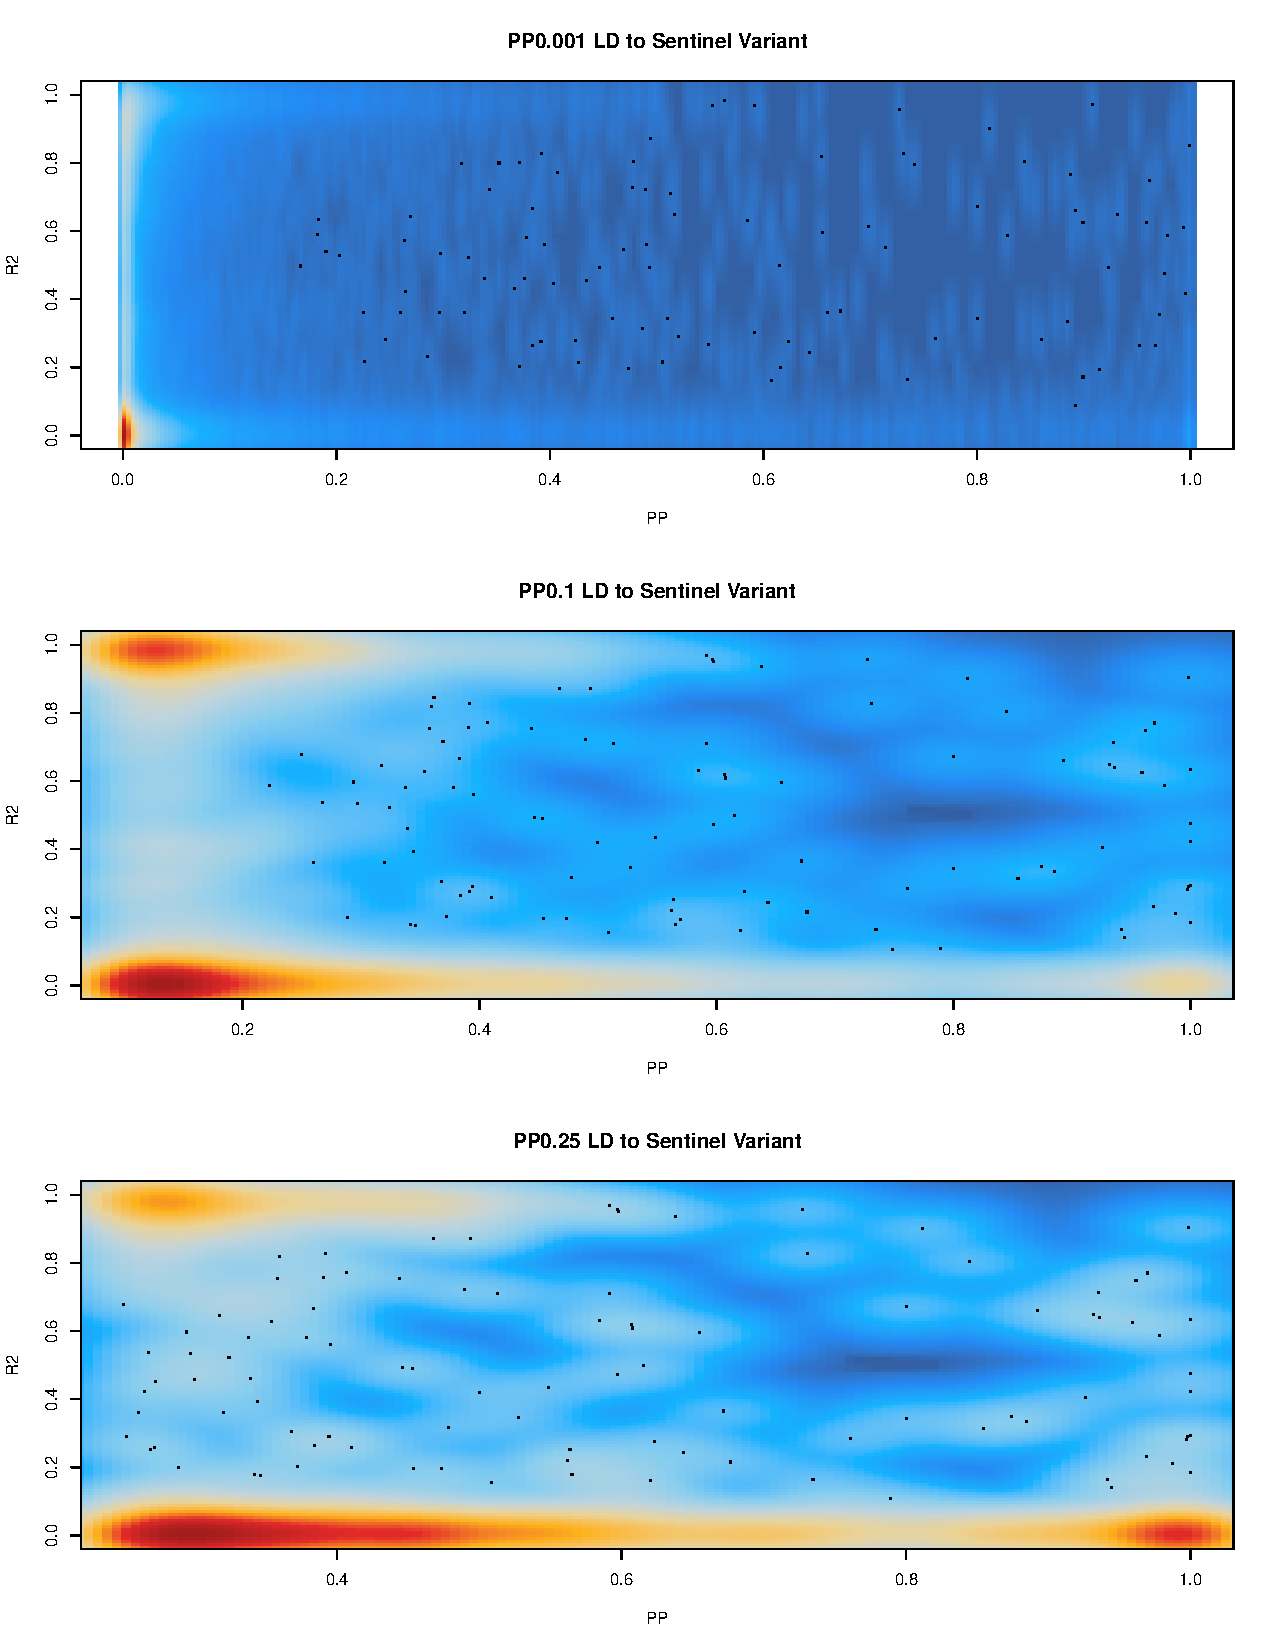
\includegraphics[width=\linewidth]{staticFigures/LDtoSentinel_PPcomparison.pdf}
\caption{Sample embedding of figure in document.}
\end{figure} 

\end{enumerate}


\end{document}
